\section{Cloud Infrastruktur}

Das Trainieren eines \textit{Deep Learning} Modells ist gerade bei großen CNN Architekturen rechenaufwendig. Tensor Operationen wie Matrixmultiplikationen und Konvolutionen erfordern im Rahmen des maschinellen Lernens hohe Parallelisierung und Taktfrequenzen, um in absehbarer Zeit gute Ergebnisse zu liefern. Die Rechenkapazität normaler Desktop-PCs reicht meist nicht aus, um performantes \textit{Deep Learning} betreiben zu können. 

Abhilfe bieten Software-as-a-Service (SaaS) bzw. Platform-as-a-Service (PaaS) Angebote wie \textit{Amazon SageMaker}, \textit{Google Cloud Platform Cloud AI} oder \textit{Azure ML Services} oder aber auch Start-ups wie \textit{FloydHub}. Diese bieten Infrastruktur in unterschiedlichen Zonen je nach Standpunkt der Rechenzentren zum Trainieren an sowie eine Plattform zum Verwalten der \textit{Deep Learning} Prozesse. 

\subsection*{Trainingshardware}

Gerade GPUs bieten sich aufgrund ihres hohen Parallelisierungsvermögens gegenüber herkömmlichen CPUs an. Insbesondere \textit{NVIDIA} nimmt hierbei eine Vorreiterrolle in der Produktion von Server-GPUs ein. Die \textit{Compute Unified Device Architecture} (CUDA) von \textit{NVIDIA} ermöglicht als Programmiermodel und parallele Computing Plattform das Auslagern von Rechenprozessen auf GPUs. Das \textit{CUDA} Toolkit beinhaltet GPU beschleunigte Bibliotheken, einen Compiler, Entwicklungswerkzeuge sowie die eigentliche \textit{CUDA} Laufzeit und wird von vielen \textit{Deep Learning} Bibliotheken genutzt, wie z.B. \textit{PyTorch} \cite{NVIDIA.20200209, PyTorch.20200209}. Hauptvergleichskriterien zwischen GPUs sind hierbei der Grad der möglichen Parallelisierung und die reine Rechenleistung im Verhältnis zum Stromverbrauch.

Neben GPUs existieren seit 2015 die von Google entwickelten \textit{Tensor Processing Units} (TPUs). Diese sind speziell entwickelte, anwendungsspezifische integrierte Schaltung (engl.: \textit{Application-Specific Integrated Circuit}) (ASIC) für Arbeitslasten im maschinellen Lernen \cite{GoogleCloud.20200209b}.

Eine weitere Steigerung versprechen Microsofts Field Programmable Gate Arrays (FPGAs), die allerdings nicht weiter im Rahmen dieser Arbeit betrachtet werden sollen \cite{KarlFreund.20170828}.

\subsection*{Amazon Web Services SageMaker}

\textit{Amazon Web Services} (AWS) bietet mit \textit{SageMaker} eine integrierte Plattform zum Trainieren und Bereitstellen von \textit{Deep Learning} Modellen. Zentrales Alleinstellungsmerkmal ist das einheitliche Toolset, in dem alle Arbeitsprozesse rund um ein \textit{Deep Learning} Modell integriert abgebildet werden können. Es ist somit nicht mehr nötig, unterschiedliche Tools und Arbeitsabläufe zusammenfügen, was zuvor zeitaufwändig und fehleranfällig war \cite{AmazonWebServices.20200314}.

Außerdem bietet \textit{AWS SageMaker} die ersten vollständig integrierte Entwicklungsumgebung für Machine Learning, \glqq Amazon SageMaker Studio\grqq{}. Zum Erstellen der \textit{Deep Learning} Modellen werden sogenannte \textit{Amazon Sagemaker Notebooks} genutzt, eine Ableitung klassischer \textit{Jupyter Notebooks}. Unterstützte Frameworks sind TensorFlow, PyTorch, Apache MXNet, Chainer, Keras, Gluon, Horovod, Scikit-Learn und Deep Graph Library \cite{AmazonWebServices.20200314}. 

\textit{AWS SageMaker} bietet verschiedene Instanztypen an, die sich je nach Anzahl an vCPUs und GPUs unterscheiden. Auch der vorhandene Arbeitsspeicher, Grafikkartenspeicher und die Netzwerkleistung kann durch die Vielzahl an angebotenen Instanzen nach individuellen Bedürfnissen gewählt werden \cite{AmazonWebServices.20200314b}.

\subsection*{Google Cloud Platform AI Platform}

\textit{AI Platform} ist das Konkurrenzprodukt zu \textit{AWS SageMaker} von der \textit{Google Cloud Platform} (GCP). Die Plattform bietet ebenso verschiedene Komponenten für das \textit{Deep Learning} an. Hierzu gehören \textit{AI Platform Notebooks}, ein Dienst mit einer integrierten JupyterLab-Umgebung, \textit{Deep Learning} Virtual Machines (VM) mit vorinstalierten \textit{Deep Learning} Frameworks, verteiltes Training mit automatischer Hyperparameter-Abstimmung durch den \textit{AI Platform Training} Dienst oder \textit{AI Platform Prediction} zum Bereitstellen trainierter Modelle \cite{GoogleCloudPlatform.20200314}. 

Hervorzuheben sind allerdings Googles TPU Hardwarebeschleuniger, die für Projekte im \textit{TensorFlow} Framework für jede Instanz mobilisiert werden können. Diese Art von Spezialhardware erreicht pro TPU-Kern eine Rechenleistung von bis zu 92 TOPS \cite{HaraldBogeholz.20170406}. Werden 2048 solcher TPU-Kerne zu einem TPU-Pod zusammen geschlossen, so ergibt sich eine Rechenleistung von über 100 PetaFLOPS \cite{GoogleCloud.20200209}. Zudem ist die größere Rechenleistung gleichzeitig effizienter als herkömmliche GPUs (siehe Abbildung \ref{tpu}).

\begin{figure}[ht]
	\begin{center}
		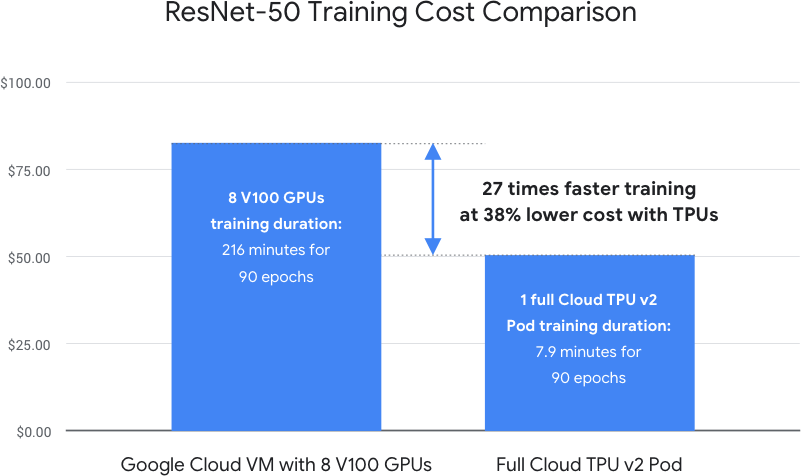
\includegraphics[width=14cm]{Bilder/tpu_comparison.png} 
		\caption[Vergleich V100 - TPU Pod]{Vergleich V100 - TPU Pod \cite{GoogleCloud.20200209b}}
		\label{tpu}
	\end{center}
\end{figure}

TPUs sind also darauf ausgelegt, ein optimales Preis-/Leistungsverhältnis beim Trainieren von \textit{Deep Leaning} Modellen zu erreichen \cite{GoogleCloudPlatform.20200314}.

\subsection*{Google Colab}

\textit{Google Colaboratory}, kurz \textit{Google Colab}, ist eine kostenfreie, cloudbasierte \textit{Jupyter Notebook} Umgebung von Google. Dokumente, die in Google Colab erstellt werden, werden automatisch mit \textit{Google Drive} synchronisiert. Die Laufzeit ist frei konfigurierbar zwischen Python 2 und 3 bzw. zwischen einfachem CPU, GPU oder TPU Computing. Nachteil an dem kostenfreien \textit{Google Colab} ist, dass zugewiesene Hardwareresourcen mit weiteren Nutzern geteilt werden müssen und so nicht die volle Rechenleistung für den individuellen Entwickler zur Verfügung stehen \cite{GoogleColaboratory.20200314}. 

Auch können keine längerfristigen Trainingsjobs ausgeführt werden, ohne dass nach 90 Minuten der Client von dem zugewiesenen Server getrennt wird \cite{GoogleCloud.20200314}.

\subsection*{Microsoft Azure}

\textit{Microsoft Azures} Angebot für \textit{Deep Learning} in der Cloud ist zunächst wenig transparent. Sie bieten ebenso wie Amazon und Google das Trainieren und Bereitstellen von \textit{Deep Learning} Modellen an und zudem eine einige DevOps Landschaft für solche Arbeitsprozesse. Auch werden Frameworks wie \textit{TensorFlow} oder \textit{PyTorch} unterstützt sowie das Programmieren in \textit{Jupyter Noteboks} \cite{MicrosoftAzure.20200314}.

\subsection*{FloydHub}

FloydHub, ein kalifornisches Start-up, bietet eine Data-Science Plattform zum Trainieren und Bereitstellen von \textit{Deep Learning} Applikationen. FloydHub erlaubt es Anwendern, sich auf reines \textit{Deep Learning} zu konzentrieren, während es die Arbeit rund um den \textit{Deep Learning} Lebenszyklus abnimmt. Hierzu gehört das Bereitstellen der entsprechenden Hardware, das Installieren von Treibern oder das Integrieren verschiedener \textit{Deep Learning} Bibliotheken, wie \textit{TensorFlow}, \textit{PyTorch} oder \textit{Keras} \cite{FloydHub.20200215}. 

Mit Hilfe des von FloydHub bereitgestellten Command Line Interfaces (CLI) kann ein lokales Projekt zu einem FloyHub Projekt initialisiert werden. Anschließend können anhand einer Konfigurationsdatei Einstellungen über das Training spezifiziert werden (siehe Listing \ref{floydhub:FloydHub}). Alternativ können diese auch über das CLI festgelegt werden. 

\lstset{language=XML}
\lstinputlisting[
label=floydhub:FloydHub,
caption=Konfigurationsdatei zum Trainingsjob auf FloydHub,
captionpos=b,
firstline=1,
lastline=9
]{Quellcode/floyd.yml}

Hierbei kann zwischen der K80 (gpu) oder der V100 (gpu2) GPU für das Training gewählt werden. Auch die \textit{Deep Learning} Laufzeitumgebung muss spezifiziert werden. Bei Bedarf auch zusätzliche Bibliotheken in einer \textit{floyd\_requirements.txt}-Datei zur Installation mit angegeben werden. Anschließend muss der Datensatz referenziert werden, mit dem das Modell trainiert werden soll. 

Dieser Datensatz wird separat hochgeladen, da sich dieser im Gegensatz zum Programmcode nur selten ändert. FloydHub implementiert auf seiner Plattform eine Art Pfadsystem, unter dem Datensätze und Projekte abgespeichert werden. Diese Pfade werden in der Konfigurations-Datei zur Referenzierung genutzt. Um auch im Programmcode auf den Datensatz zuzugreifen, muss ein Mountname definiert werden. In obigen Beispiel wird dem Datensatz unter Verzeichnis \textit{<username>/datasets/smartwarehousessd/3} der Mountname \textit{ssd} gegeben. Das Verzeichnis zum Einlesen der Daten ist anschließend im Code unter \textit{/floyd/input/ssd/} erreichbar. 

Mit dem CLI Befehl \textit{floyd run} wird der Programm Code auf die Plattform hochgeladen und der in der Konfigurationsdatei angegebene Befehl ausgeführt. Daraufhin wird ein Job erstellt, versioniert und ausgeführt. Während der Job ausgeführt wird, wird dem Nutzer ein Einblick in die Konsolenausgabe gewährt sowie in Metriken zur Hardwareauslastung. In der Jobhistorie kann im Nachhinein jeder Job mit dem damals aktuellen Programmcode und Datensatz eingesehen werden. Auch Datensätze werden versioniert. Schreibrechte sind auf das Verzeichnis \textit{/floyd/home} begrenzt, hier können Zwischenspeicherpunkte des Modells abgelegt werden. 

Neben klassischen Trainingsjobs können \textit{Deep Learning} Modelle auch ganz einfach in \textit{Jupyter Notebooks} erstellt werden. Hierzu muss in einem Projekt ein Workspace angelegt werden.

